% Crucial Preamble
\documentclass[12pt,letterpaper]{article} \usepackage{amsmath} \usepackage{graphicx}  \usepackage{longtable}  \usepackage{amssymb}
%\usepackage[margin=0.7in]{geometry}

\usepackage[left=1.3cm,top=2.5cm,right=1.3cm,bottom=2.5cm,bindingoffset=0cm]{geometry}


% Extra Preamble
\usepackage{fancyhdr} \usepackage{enumitem} \usepackage{float} \usepackage{soul}
\usepackage{multicol} \usepackage[compact]{titlesec}


% frames with display breaks
\usepackage{mdframed}
\allowdisplaybreaks

% change spacing
\usepackage{setspace}
\setlength{\parskip}{0.4\baselineskip}

% Remove paragraph indentation
\setlength{\parindent}{0pt}

% Reduce space before and after section headings
\titlespacing*{\section}{0pt}{0.1\baselineskip}{0.2\baselineskip}

% changes font
%\renewcommand{\familydefault}{\sfdefault}

% adds header and footer
\pagestyle{fancy}
\fancyhead{} \fancyhead[C]{Whole Year Cheat Sheet} \fancyhead[L]{MAT1322} \fancyhead[R]{Owen Daigle}
\fancyfoot{} \fancyfoot[C]{\tiny{PRAISE THE ABSOLUTE}} \fancyfoot[R]{ \thepage }

\begin{document}

    \thispagestyle{empty}
    \begin{center}
        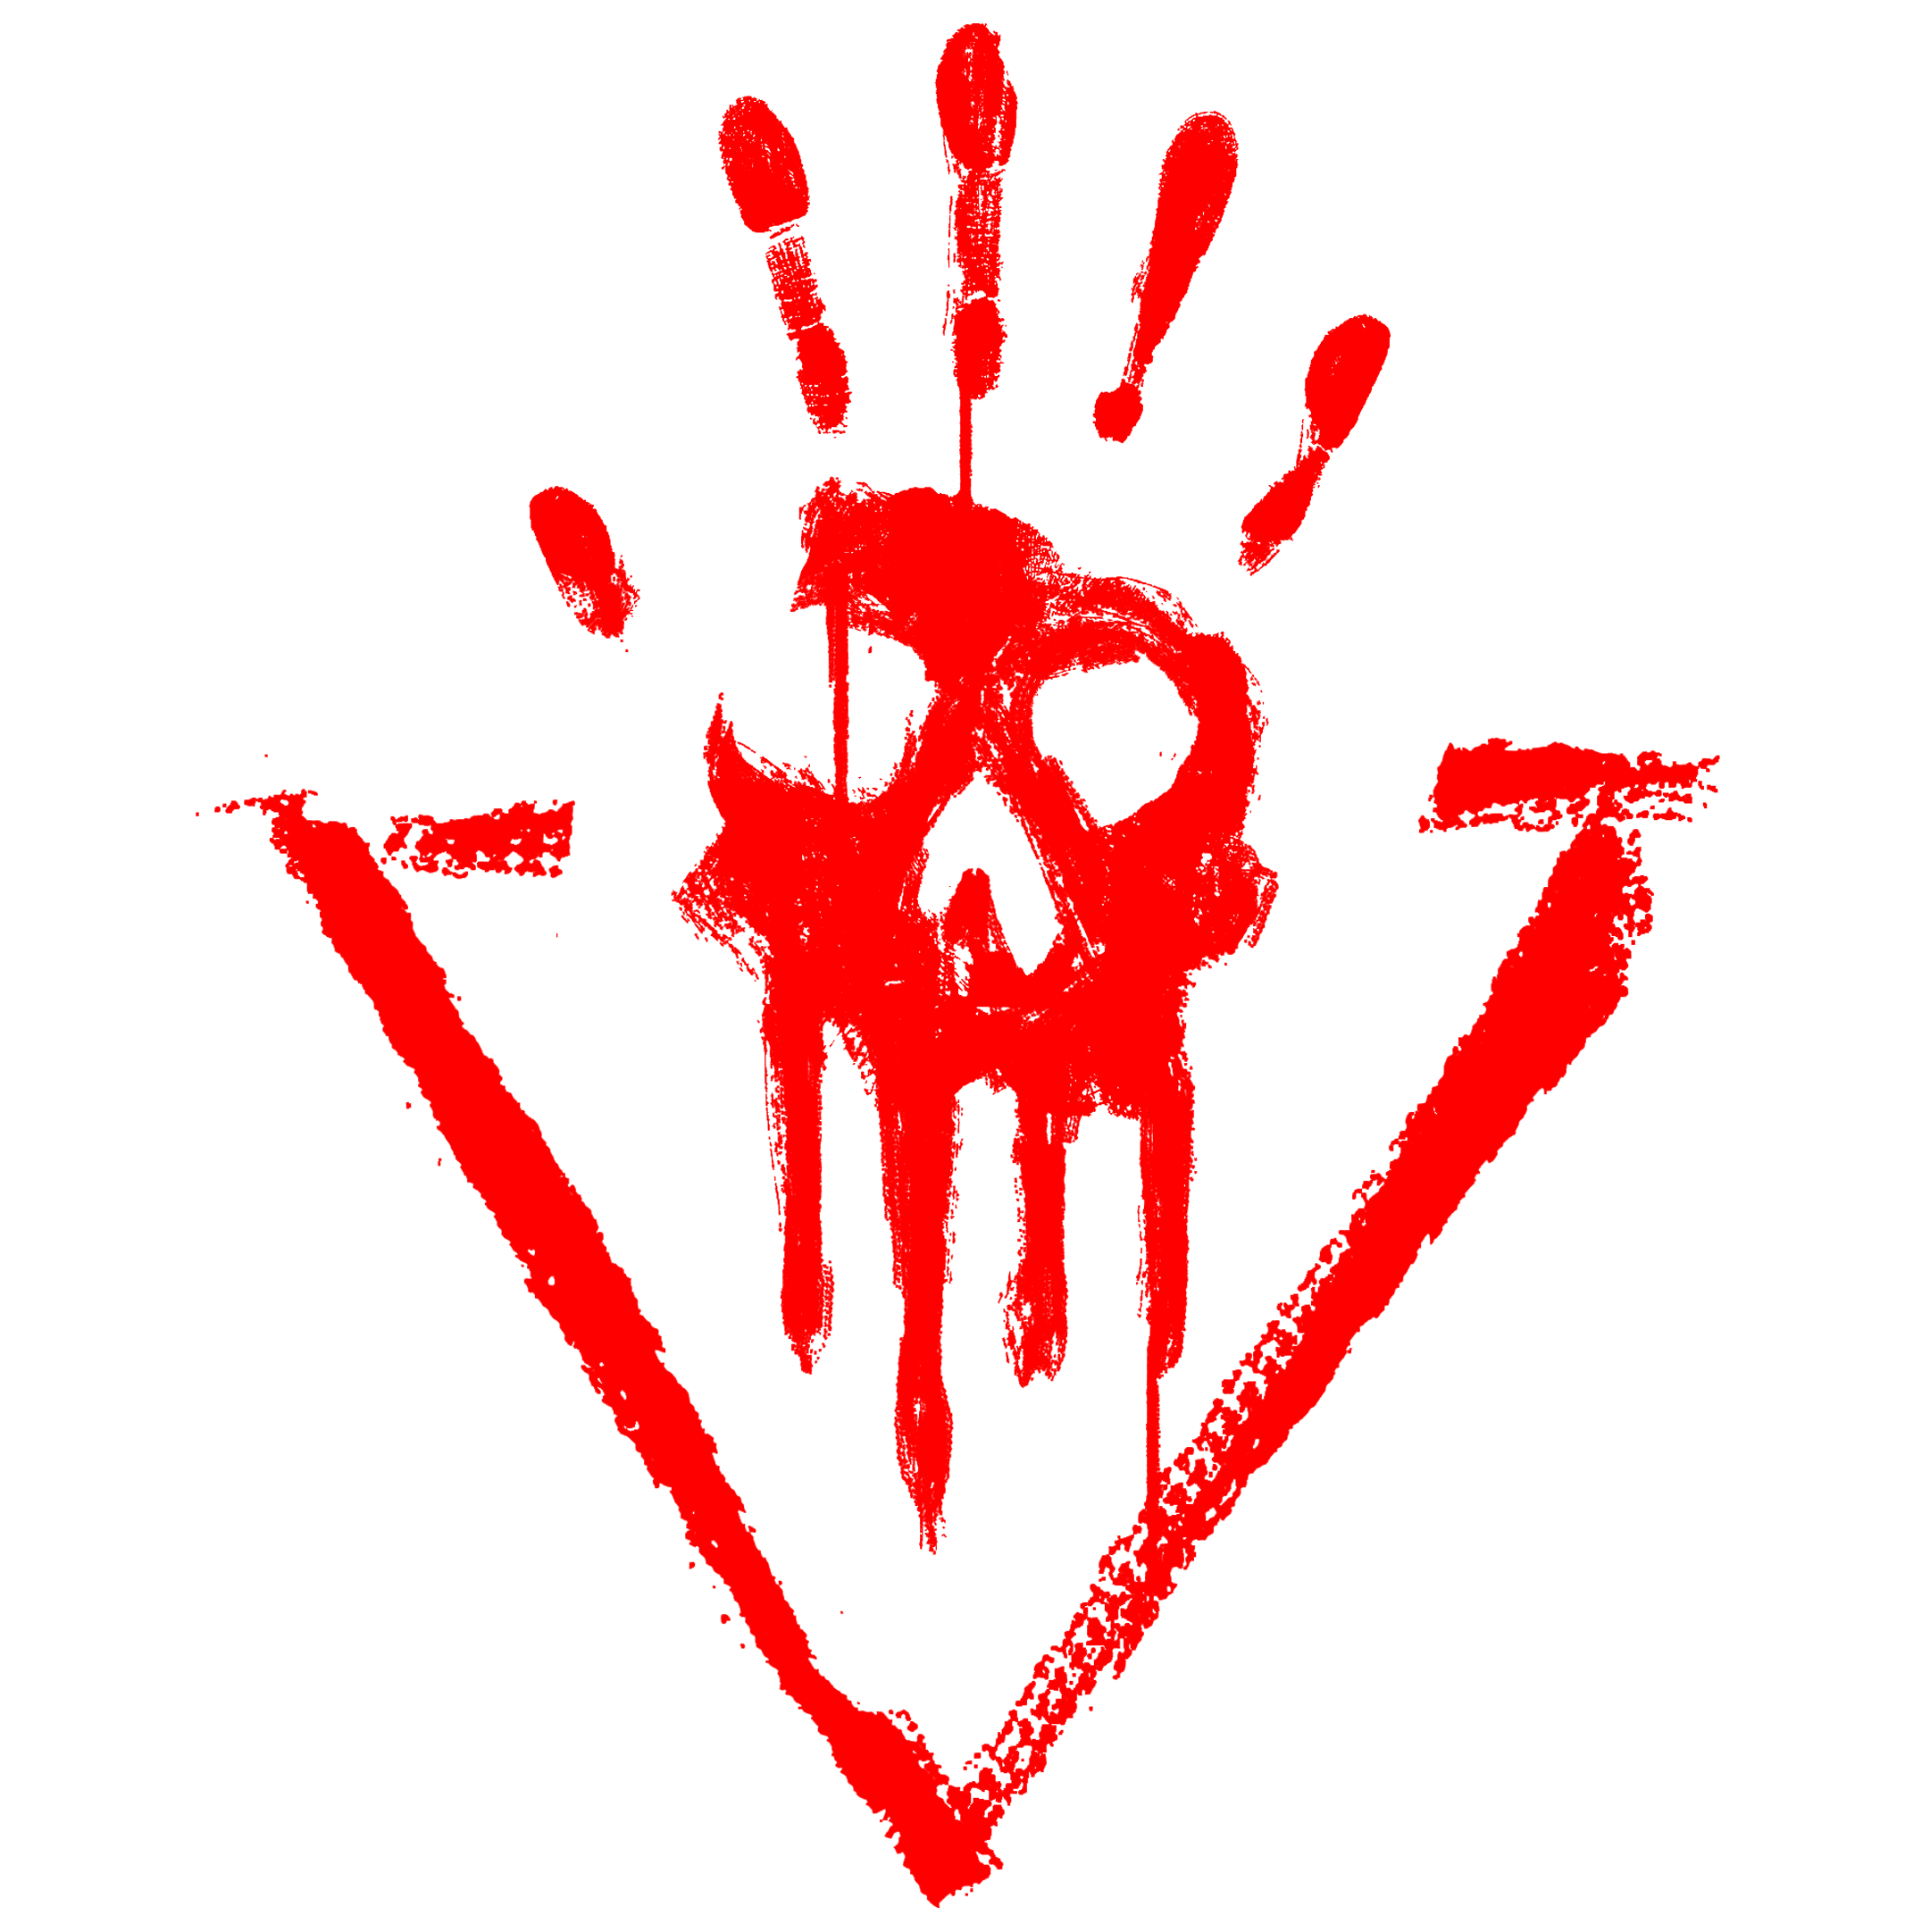
\includegraphics[width=0.12\linewidth]{abs.png}\\
        \vspace{2em}
        \Large\textbf{MAT 1322 Cheat Sheet} \\
        \vspace{0.5em}
        \small{Winter 2024} \\
        \small{University of Ottawa} \\
        \small{Owen Daigle}
    \end{center}

    \pagebreak

    \begin{spacing}{0}
    \tableofcontents
    \end{spacing}

    \pagebreak
    
    % doc begins here

    \section{Improper Integrals}
    An Integral is called \emph{improper} if it either has $\infty$ in either of its bounds, or it is undefined at a point in its bounds. 

    To evaluate an improper integral, we take the limit of said integral as $t\to\infty$ with $t$ as the improper bound, then we compute the integral and then the limit. 

    An integral is called convergent if it converges on a finite value. Otherwise, it is called divergent. 

    We can use the comparison test to determine whether an improper integral converges or diverges. 
    
    This basically says, if there are 2 integrals with one bigger than the other, then the following must be true:
    \begin{enumerate}
        \item If the larger one converges, then the smaller one must converge. 
        \item If the smaller one diverges, then the larger one must diverge. 
    \end{enumerate}

    \begin{mdframed}
        \textbf{Ex. } Evaluate the following integral's nature:
        \begin{align*}
            \int^{\infty}_ {-\infty} \frac{1}{1+x^2} dx
        \end{align*}
        
        The actual integral part looks simple. But it is a double improper integral. To solve this, we will break it up into 2 parts. The part above 0, and the part below 0. If both converge to the same value, then it is convergent. otherwise, divergent.

        \begin{align*}
            & \int^0_{-\infty} \frac{1}{1+x^2} dx & \int^{\infty}_0 \frac{1}{1+x^2} dx\\
            &=\lim_{t\to -\infty} \int^0_t \frac{1}{1+x^2} dx &= \lim_{t\to \infty} \int_0^t \frac{1}{1+x^2} dx\\
            &= \lim_{t\to -\infty} \left[\arctan(x)\right]_t^0 &= \lim_{t\to\infty} \left[\arctan(x)\right]^t_0\\
            &= 0 - \frac{-\pi}{2} = \frac{\pi}{2} &=\frac{\pi}{2}-0
        \end{align*}
        Since both parts converge to the same number, then the entire integral converges as well.
    \end{mdframed}

    \section{Integral Applications}
    In these problems, we often are given a problem, and we need to look at what variables we have, and of those, which ones are changing, and which are constant. The constant ones are easy, but the changing ones will need to be integrated. Since we can only integrate one variable, we often need to get one variable in terms of other variables. 

        \subsection{Areas}
        To find the area between 2 functions, we take the integral of the difference of the 2 functions.

        \textbf{Suppose} $f>g$ and $a,b\in\mathbb{R}$:
        
        \textbf{Then} the area of the region bounded by $a, b, f, g$ is:
        \begin{align*}
            A = \int ^b_a \left(f(x)-g(x)\right)dx
        \end{align*}

        \subsection{Volumes}
        To find the volume of a 3d shape bounded by 2 functions $f$ and $g$, we take infinitely many slabs of width $\Delta x$ and we find their area. Then we can integrate the area between the points of intersection of $f$ and $g$.
            \subsubsection{Method of Slices (Cross Sections)}
            Using cross sections, we either create infinitely many washers, or disks where the disk is a solid, and the washer has a hole in the middle. 
            \begin{align*}
                V=\int^b_a \left(\pi \left(R(x)^2 -r(x)^2 \right)\right)dx
            \end{align*}

            $R(x)$ is the outer radius, $r(x)$ is the inner radius (0 if we are using a disk).

            \subsubsection{Method of Shells}
            The method of shells is useful if we are rotating about a vertical line with a large hole in the middle.
            We use the following formula. $r$ is generally the line that we are rotating about, $f, g$ are functions where $f>g$. $a, b$ are the bounds of the function. Note that $|a-b|$ will be the max radius of the function. 
            \begin{align*}
                V = \int^b_a \left(2\pi\left(x-r\right)\cdot (f(x)-g(x))\right)
            \end{align*}

            \begin{mdframed}
                \textbf{Ex. } Let $S$ be the solid obtained by rotating the area enclosed by the following 2 functions around the line $x=2\pi$. Calculate the volume of this structure. 
                \begin{align*}
                    y&=\cos(x) \{0\le x\le 2\pi\}\\
                    y&=2-\cos(x) \{0\le x\le 2\pi\}
                \end{align*}

                First we need to draw this out. I know that the 2 functions will create an enclosed area that will be rotated around the line of $x=2\pi$. 

                \begin{figure}[H]
                    \centering
                    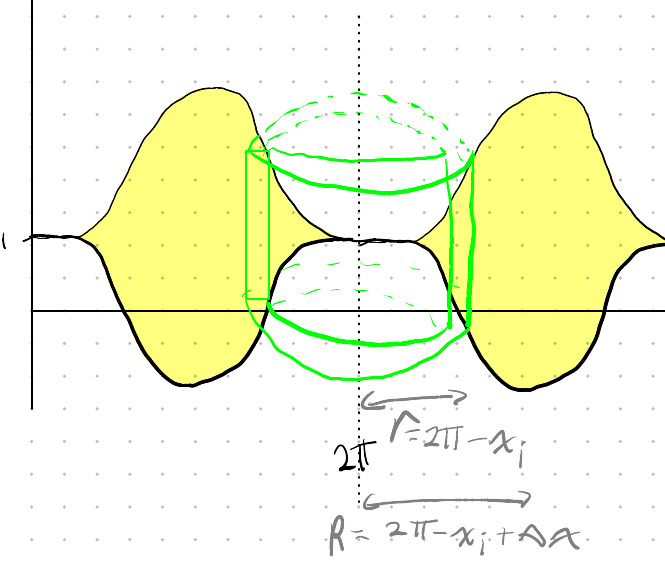
\includegraphics[width=0.5\linewidth]{ex4.png}
                \end{figure}

                We will be using the method of shells for this.

                We can see that the height at a point $x$ is just the top function - the bottom function. $2-\cos(x) - \cos(x) = 2-2\cos(x)$.

                The radius also changes with $x$. It will be $2\pi -x$

                Putting this into the method of shells equation, we get:
                \begin{align*}
                    \int^{2\pi}_0 2\pi (2-2\cos(x))(2\pi =x)dx = \text{CALC}
                \end{align*}

            \end{mdframed}

        \subsection{Work}
        Work is given by the formula $W=Fd$ where $F$ is the force, and $d$ is the displacement.
            \subsubsection{Work in Tanks}
            If we need to pump water out of the tank we use the following work formula:
            \begin{align*}
                W = \int_a^b V\rho gd
            \end{align*}
            $V$ is the volume, $\rho$ is the density ($\rho_{water} = 1000$), $g$ is gravity, and $d$ is the displacement that the slab of water has to move (depends on $x$).

            \begin{mdframed}
                \textbf{Ex. } A spherical reservoir has a radius of 5m. It is filled up to 8m with water. Compute  the work to pump the water up to 2m above the top of the resevoir. 

                We start with the equation for work.
                \begin{align*}
                    W_i = Fd = mgd = V\rho gd = (\pi r_i^2\Delta x)\rho gd_i
                \end{align*}
                We see that the radius ($r$) and the distance that the water is required to be pumped ($d$) change with the amount of remaining water in the tank.

                So we need to get $r$ and $d$ in terms of $x_i$. 

                First we draw the situation. 

                \begin{figure}[H]
                    \centering
                    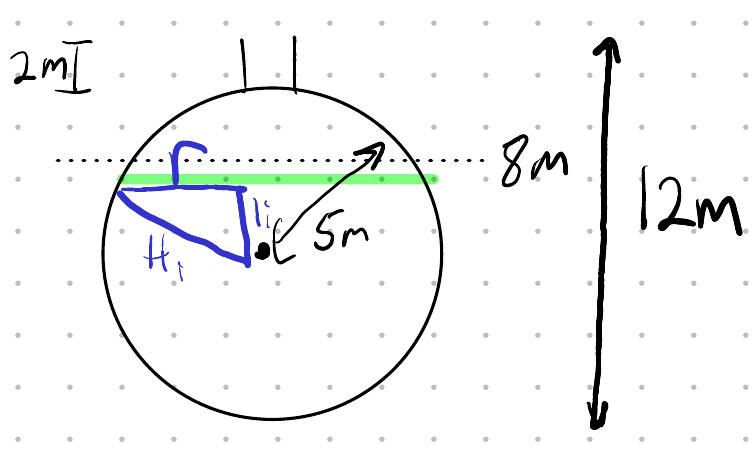
\includegraphics[width=0.4\linewidth]{ex5.png}
                \end{figure}

                We know that $H_i, r_i, l_i$ are related, and we know $H_i = 5$. So if we find $l_i$, then we know $r_i$. 

                We define that $x_i$ is the point that we are integrating. It is 0 at the bottom, and 8 at the top of the water. 

                We see that $l_i$ is equal to the difference between the current height of the water, and $H_i$. So, $l_i = |x_i - 5| \implies r_i = \sqrt{25-(x_i - 5)^2}$.

                For $d$ in terms of $x_i$, we know that the amount of water needing to be pumped is simply the total height - the current height $12 - x_i$.

                Subbing all this injto the original equation, we get:
                \begin{align*}
                    W = \int^8_0 9.8 \cdot 1000 \cdot (\pi \cdot (\sqrt{25-(x-5)^2}))\cdot (12-x) dx = \text{CALC}
                \end{align*}
            \end{mdframed}

            \subsubsection{Work on Ropes}
            The force is given by the weight of the rope, and because the rope has a constant weight throughout the rope, then we just do the integral of the weight for one unit times $x$.

            \subsubsection{Work on Springs}
            We just integrate the product of the spring constant $k$ times $x$. 

        \subsection{Average Value}
        We use the following simple formula to calculate the average value of a function on $[a,b]$.
        \begin{align*}
            F_{avg} = \int_a^b \left(\frac{1}{b-a} f(x)dx\right)
        \end{align*}

        \subsection{Arc Length}
        We use the following simple formula to calculate the arc length of a curve on an interval $[a,b]$.
        \begin{align*}
            L = \int^b_a \left(\sqrt{1+f'(x)^2}\right)dx
        \end{align*}

        \subsection{Hydrostatic Force}
        To calculate the hydrostatic force, we use the following formula:
        \begin{align*}
            F = \int^b_a \rho Adg\cdot dx
        \end{align*}
        $\rho$ is the density, $g$ is gravity. $A$ is the area which is changing (width times $\Delta x$). $d$ is the distance between the surface of the water and the current slab ($x$)

        \begin{mdframed}
            \textbf{Ex. } Assume a vertical plate is submerged 1m under the water where the plate has the following dimensions:

            \begin{figure}[H]
                \centering
                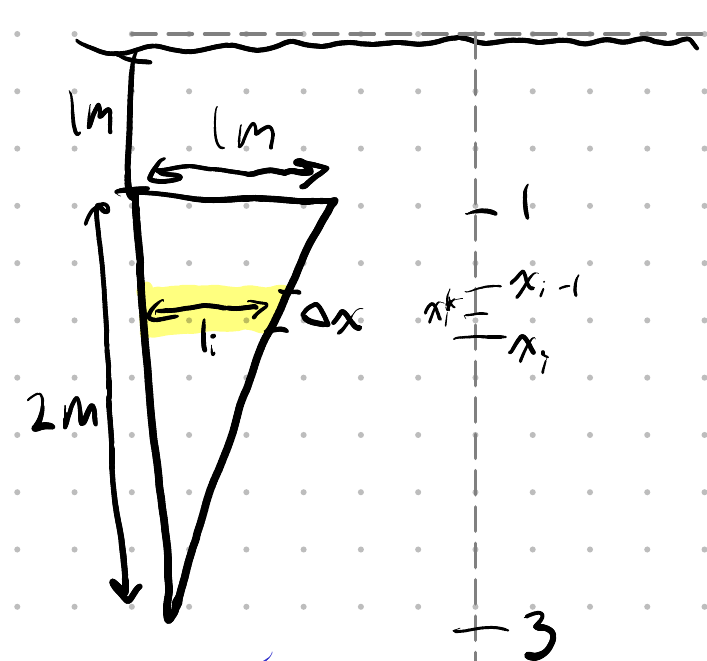
\includegraphics[width=0.4\linewidth]{ex6.png}
            \end{figure}

            We let $0$ be the top of the liquid. 

            We need to find the area, and the distance between the current slab and the top. $d=x$.

            The area is more complex. The area of a rectangular slab of width $\Delta x$ is $A = \Delta x \cdot l_i$. We do not know $l_i$, but we can find it using similar triangles. 

            We see 2 triangles. One of them is the whole shape with side lengths of 1m, and 2m. The other one is the smaller one with height of $3-x_i$, and width of $l_i$. We set up the following similar triangle equation:
            \begin{align*}
                \frac{l_i}{3-x_i} = \frac{1}{2} \implies l_i = \frac{3-x_i}{2}
            \end{align*}

            And now we can just sub into the force equation. 

            \begin{align*}
                F = \rho A d g = 1000\cdot 9.81\cdot \int^3_1 \frac{3-x}{2} \cdot x dx = \text{CALC}
            \end{align*}

        \end{mdframed}

        \subsection{Center of Mass}
        To calculate the center of mass of an area, we use the following coordinates for the x and y coordinates.
        \begin{align*}
            &\overline{x}=\frac{\int^b_a x(f(x)-g(x))dx}{A} & \overline{y}=\frac{\int^b_a \frac{1}{2}(f(x)^2 - g(x)^2)}{A}
        \end{align*}

        To get the moment equations, it is just the center of mass, but without the demonator of area. Instead, it is multiplied by the density $\rho$.

    \section{Differential Equations}
    A differentiable equation is an equation that involves at least a derivative of an unknown function. 
    
    A differentiable equation is called seperable if it can be written as: $\frac{dy}{dx} = f(x)\cdot g(y)$.

    \begin{mdframed}
        \textbf{Ex. } Solve the following DE: $\frac{dy}{dx} = xy\cos(x^2)$ at $y(0) = 2$

        First we will get all the $y$s on one side, and the $x$s on the other.
        \begin{align*}
            &\implies \frac{dy}{y} = x\cos(x^2)dx\\
        \end{align*}
        Now we integrate both sides
        \begin{align*}
            &\implies \int \frac{dy}{y} = \int x\cdot \cos(x^2) dx\\
        \end{align*}
        Using u substitution with $ u = x^2, du = 2xdx$
        \begin{align*}
            &\implies \ln|y| = \frac{-\sin(x^2)}{2}+C\\
        \end{align*}
        Subbing in the point, we get:
        \begin{align*}
            &\implies \ln(2)=\frac{\sin(0)}{2}+C \implies C=\ln(2)\\
            &\ln|y| = \frac{-\sin(x^2)}{2} + \ln(2)\\
            &|y| = e^{\frac{-\sin(x^2)}{2}+\ln(2)} \implies y = \pm e^{\frac{-\sin(x^2)}{2}+\ln(2)}
        \end{align*}
    \end{mdframed}

        \subsection{Applications of Differential Equations (DEs)}
            \subsubsection{Growth / Decay}
            We have the following 3 formulas which we can use to solve equations.
            \begin{align*}
                \frac{dp}{dt}=kp\\
                P(t)=P(0)e^{kt}\\
                \frac{\frac{dp}{dt}}{P}=k
            \end{align*}
            $k$ is a constant, $P(0)$ is the initial population, and $P(t)$ is the population at time $t$. 

            \subsubsection{Cooling / Heating}
            This is similar to Growth / Decay problems, but uses the following formula.
            \begin{align*}
                T(t)=A+(T(0)-A)e^{kt}
            \end{align*}
            $A$ is the ambient temperature, $T(0)$ is the initial temperature, $T(t)$ is the temperature at time $t$, and $k$ is the constant.

            \subsubsection{Mixing}
            This has a very simple formula. 
            \begin{align*}
                \frac{dy}{dt}=\text{Rate In} - \text{Rate Out}
            \end{align*}

    \section{Sequences}
    A sequence is an \emph{ordered} list of numbers such as\\
    \begin{align*}
        &{1,2,3,4,5,...,n} &\text{or      } & a_n = \frac{2}{3+n}
    \end{align*}

    We can find whether a sequence is convergent or divergent by taking its limit as $n\to\infty$. If this is a number, it is convergent, otherwise, it is divergent.

    \section{Series}
    Given a sequence $\{a_n\}_{n \ge 0}$ we can construct a series $\sum _{n=0} ^{\infty} a_n$:
    \begin{align*}
        &s_0 = a_0\\
        &s_1 = a_0 + a_1 \\
        &s_2 = a_0 + a_1 + a_2\\
        &\vdots\\
        &s_n = a_0 + a_1 + \dots + a_n
    \end{align*}

    This series can either converge on one number, or diverge to $\pm \infty$.

    \section{Series Tests}
    We use these tests, sometimes, but \emph{not necessarily} in this order, to determine the nature (Convergent or Divergent) of a given series. 

        \subsection{Divergence Test}
        Consider $\sum ^{\infty} _ {n=1} a_n$.
        \textbf{If} $\lim_{n\to\infty} a_n \ne 0$, \textbf{then} $\sum ^{\infty} _ {n=1} a_n$ is Divergent

        \subsection{P Series}
        Consider a series in the following form:
        \begin{align*}
            \sum^\infty _{n=0} \frac{1}{n^p}
        \end{align*}

        If $p\le 1$, the series is divergent. If $p>1$, the series is convergent.

        \subsection{Geometric Series}
        Consider a series in the following form:
        \begin{align*}
            a, ar, ar^2, ar^3, ..., ar^n, ar^{n+1}, ...
        \end{align*}
        We call $a$ the first term, and $r$ the common ratio.
        This type of series is convergent if $r\in(-1,1)$.

        We can find the sum of said series using the following equation:
        \begin{align*}
            s_n = \frac{a}{1-r} \cdot (1-r^n)
        \end{align*}

        \begin{mdframed}
            \textbf{Ex.} Is $\sum^{\infty}_{n=1}6^2 \cdot \frac{3^n}{4^{n+1}}$ convergent? If so, find its sum.

            We see that this is in the general form of a geometric series especially if we do:
            \begin{align*}
                a_n = 6^2 \cdot \frac{3^n}{4^{n+1}} = 6^2 \cdot \left(\frac{3^n}{4^n}\right) \cdot \frac{1}{4} = 9\cdot\left(\frac{3}{4}\right)^n
            \end{align*}

            Evidently we can see that $r=\frac{3}{4} \in (-1,1)$ so it is convergent. 

            Using the sum formula, we get:
            \begin{align*}
                \frac{a}{1-r}(1-r^n) = \frac{9}{1-\left(\frac{3}{4}\right)}\left(1-\left(\frac{3}{4}\right)^n\right) = 36.3
            \end{align*}
        \end{mdframed}

        \subsection{Telescopic Series}
        Consider a series in the following form, denoted a telescopic series:
        \begin{align*}
            \sum _ {n=1} ^{\infty} \frac{1}{n+A} - \frac{1}{n+B}
        \end{align*}
        Then, after at least $k$ terms are written out, where $k$ is $|B-A|+1$, some terms will be cancelled out and we will be left with $k$ finite terms, and $k$ terms with $n$.

        These can be made by taking a series in the following form and breaking it into 2 parts using the method of partial fractions.
        \begin{align*}
            \sum _ {n=1} ^{\infty} \frac{1}{An^2+Bn+C}
        \end{align*}

        \begin{mdframed}
            \textbf{Ex.} Find the sum of this telescopic series: $\sum^{\infty}_{n=1}\frac{1}{n^2+3n+2}$

            I can break this up using partial fractions. 
            \begin{align*}
                \frac{1}{(n+2)(n+1)} = \frac{A}{n+2} + \frac{B}{n+1}\\
                1 = A(n+1) + B(n+2)\\
                1 = An + A + Bn + 2B\\
                1 = A + 2B, 0 = A + B \implies A = -1, B = 1
            \end{align*}
            So now I have:
            \begin{align*}
                \sum^{\infty}_{n=1} \left(\frac{1}{n+1} - \frac{1}{n+2}\right)
            \end{align*}
            Now I can actually write out at least the first $|1-2|+1=2$ terms (although I will do 3 to show the pattern) and then cancel many terms out. 

            \begin{align*}
                \left(\frac{1}{2}-\frac{1}{3}\right) + \left(\frac{1}{3}-\frac{1}{4}\right)+\left(\frac{1}{4}-\frac{1}{5}\right) + ... + \left(\frac{1}{n+1}-\frac{1}{n+2}\right)
            \end{align*}
            I see that the $\frac{-1}{3}$ cancels out with $\frac{1}{3}$, and the $\frac{-1}{4}$ with the $\frac{1}{4}$. I can then see that a pattern appears. All will be canceled except for:
            \begin{align*}
                \frac{1}{2} - \frac{1}{n+2}
            \end{align*}

            Then as $n\to\infty$, it becomes $\frac{1}{2}$.
        \end{mdframed}

        \subsection{Comparison Test (CT)}
        Assume the series $\sum_{n=0}^{\infty}a_n, \sum_{n=0}^{\infty}b_n$ have \emph{positive} terms.
        
        \begin{enumerate}
            \item \textbf{If} $a_n \le b_n$, and $\sum_{n=0}^{\infty}b_n$ is convergent, \textbf{then} $\sum_{n=0}^{\infty}a_n$ is convergent.
            \item \textbf{If} $a_n \le b_n$, and $\sum_{n=0}^{\infty}a_n$ is divergent, \textbf{then} $\sum_{n=0}^{\infty}b_n$ is divergent.
        \end{enumerate}

        \subsection{Limit Comparison Test}
        Assume $\sum_{n=0}^{\infty} a_n$, $\sum_{n=0}^{\infty} b_n$ have \emph{positive} terms. 

        \textbf{If} $\lim_{n\to\infty} \frac{a_n}{b_n} = x \in (0,\infty)$, \textbf{then}  $\sum_{n=0}^{\infty} a_n$, $\sum_{n=0}^{\infty} b_n$ have the same nature. 

        \begin{mdframed}
            \textbf{Ex. } Decide the nature of $\sum^{\infty}_{n=1} \frac{1}{3^n -2}$

            We will use the limit comparison test with another simpler limit that we know converges. 
            \begin{align*}
                &a_n = \frac{1}{3^n - 2} &b_n = \frac{1}{3^n}\\
                &\lim_{n\to\infty} \frac{a_n}{b_n} = \lim_{n\to\infty} \frac{\frac{1}{3^n - 2}}{\frac{1}{3^n}} = \lim_{n\to\infty} \frac{3^n}{3^n - 2} = 1 \in (0,\infty)
            \end{align*}

            We know that $b_n$ is convergent since it is a geometric series with $r \in (-1, 1)$.

            We know that $a_n$ and $b_n$ must have the same nature due to the limit CT. Since $b_n$ is convergent, then $a_n$ must also be convergent. 
        \end{mdframed}

        \subsection{Alternating Series Test (AST)}
        A series whose consecutive terms have opposite signs is called an \emph{alternating series}.
        \begin{align*}
            \frac{1}{1} - \frac{1}{2} + \frac{1}{3} - \frac{1}{4} + \frac{1}{5} - ... = \sum^{\infty}_{n=1} (-1)^{n+1} \cdot \frac{1}{n}
        \end{align*}

        The alternating series test (AST) considers an alternating series $b_n$ where:
        \begin{itemize}[noitemsep]
            \item $b_n$ is positive
            \item $b_n$ is decreasing
            \item $\lim_{n\to\infty} b_n = 0$
        \end{itemize}
        \textbf{Then} the series is convergent.

        Basically, all we need to do is show that a function is positive, decreasing, and that as n goes to infinity, the series goes to 0, then it is convergent. 

        Recall that to show decreasing, we can find that the first derivative is negative. 

        \subsection{Root Test}
        Consider $\sum^{\infty}_{n=0}a_n$.
        
        \textbf{If} $\lim_{n\to\infty} \sqrt[n]{|a_n|} < 1 \text{\textbf{ Then }} \sum^{\infty}_{n=0}a_n \text{ is } AC \implies C$

        \textbf{If} $\lim_{n\to\infty} \sqrt[n]{|a_n|} > 1 \text{\textbf{ Then }} \sum^{\infty}_{n=0}a_n \text{ is } D$

        Generally we use this when there is an nth root that can be killed. 

        \begin{mdframed}
            \textbf{Ex.} Decide the nature of the series $\sum^{\infty}_{n=1} \frac{n^{2n}}{(1+n)^{3n}}$.

            Notice right away that there is a power of $n$ on the numerator and the demonator. This is a perfect case for the root test. 
            \begin{align*}
                \lim_{n\to\infty} \sqrt[n]{\left|\frac{n^{2n}}{(1+n)^{3n}}\right|} = \lim_{n\to\infty} \frac{n^2}{(1+n)^3} = 0 < 1 \implies AC \implies C
            \end{align*}
        \end{mdframed}

        \subsection{Ratio Test}
        Consider $\sum^{\infty}_{n=0}a_n$.
        
        \textbf{If} $\lim_{n\to\infty} \left|\frac{a_{n+1}}{a_n} \right| < 1 \text{\textbf{ Then }} \sum^{\infty}_{n=0}a_n \text{ is } AC \implies C$

        \textbf{If} $\lim_{n\to\infty} \left|\frac{a_{n+1}}{a_n} \right| > 1 \text{\textbf{ Then }} \sum^{\infty}_{n=0}a_n \text{ is } D$

        Generally we use the ratio test whenever there are powers of $n$ combined with $n!$.

        \begin{mdframed}
            \textbf{Ex.} Decide if $\sum^{\infty}_{n=1}\frac{10^n}{n!}$ is C or D.

            We use the ratio test due to the presence of the $n!$.
            \begin{align*}
                L = \lim_{n\to\infty}\left|\frac{a_{n+1}}{a_n}\right| = \lim_{n\to\infty}\left|\frac{10^{n+1}}{(n+1)!} \cdot \frac{n!}{10^n}\right| = \lim_{n\to\infty}\left|\frac{10}{n+1}\right| = \frac{10}{\infty} = 0 < 1 \implies AC \implies C
            \end{align*}

            Since the limit goes to 0, which is less than 1, the series is AC and therefore C. 
        \end{mdframed}

        \subsection{Integral Test}
        Assume $f:[1,\infty) \to \mathbb{R}$ is:
        \begin{enumerate}[noitemsep]
            \item Positive
            \item Continuous
            \item Decreasing
        \end{enumerate}
        Assume $a_n = f(n)$
        \begin{align*}
            \int_{1}^{\infty} f(x)dx \text{ is convergent } \leftrightarrow \sum_{n=1}^{\infty} a_n \text{ is convergent }\\
            \int_{1}^{\infty} f(x)dx \text{ is divergent } \leftrightarrow \sum_{n=1}^{\infty} a_n \text{ is divergent }
        \end{align*}

        We can show that it is positive and continuous easily. To show decreasing, show that $f'<0$. 

    \section{Estimation Theorums}

        \subsection{Error in Integral Test}
        Suppose $R_n = S-S_n$ represents the Error where:
        \begin{align*}
            R_n = a_{n+1} + a_{n+2} + ...
        \end{align*}

        \textbf{Then} 
        \begin{align*}
            \int_{n+1}^{\infty}f(x)dx\le R_n \le \int^{\infty}_{n}f(x)dx    
        \end{align*}

        \begin{mdframed}
            \textbf{Ex.} Estimate the sum of $\sum^{\infty}_{n=1} \frac{1}{n^3}$ by using the first 10 terms. Find the error. 
            
            To find the sum using the first 10 terms, we find $S_{10}$.
            \begin{align*}
                S \approx S_{10} = \frac{1}{1^3} + \frac{1}{2^3} + \frac{1}{3^3} + ... + \frac{1}{10^3} = 1.175
            \end{align*}

            To find the max error $R_n$, we know that it must be less than $\int^{\infty}_{n} f(x)dx$.
            \begin{align*}
                R_n &\le \int^{\infty}_{n} f(x)dx = \int^{\infty}_{10} \frac{1}{x^3}= \lim_{t\to\infty} \left(\frac{1}{-2t^2} - \frac{1}{-2(10)^2}\right)= 0+\frac{1}{200} \\
                R_n &\le \frac{1}{200} 
            \end{align*}

            This means that the error can be \emph{at most} $\frac{1}{200}$. 
        \end{mdframed}

        \begin{mdframed}
            \textbf{Ex Cont.} Using the same example from above, how many terms are needed to ensure the estimate is within $0.0005$ to $S$?

            We need to find $n$ such that $R_n \le 0.0005$. So we can just solve the same as before except with $n$ as the unknown. 
            \begin{align*}
                \int^{\infty}_{n} \frac{1}{x^3}dx &< 0.0005\\
                \lim_{t\to \infty} \left( \frac{1}{-2t^2} + \frac{1}{2n^2}\right) &< 0.0005\\
                \frac{1}{2n^2} &< 0.0005\\
                n&<31.222
            \end{align*}

            There must be at least $31.222$ terms for the error to be that small, and since we cannot have a fractional amount of terms, we round up to $32$. 
        \end{mdframed}

        \subsection{Alternating Series Estimation Theorum (ASET)}
        Assume $\sum^{\infty}_{n=1} (-1)^{n-1} b_n$ is convergent \emph{by AST}.

        \textbf{Then} let $S = \sum^{\infty}_{n=1} (-1)^{n-1} b_n$ be the sum.
        \begin{align*}
            R_n = S-S_n \\
            |R_n| < b_{n+1}
        \end{align*}

        \begin{mdframed}
            \textbf{Ex.} Consider $\sum^{\infty}_{n=1} (-1)^{n} \frac{1}{n!}$. How many terms are needeed such that the error is less than 0.01?

            First we prove that it is an AS. 
            
            It is positive since both numerator and denomonator are positive.

            The limit goes to 0 as n goes to infinity.

            To show decreasing, we can show that in general, the nth term is more than the nth + 1 term. 
            \begin{align*}
                \frac{b_{n+1}}{b_n} = ... = \frac{n!}{(n+1)!} < 1.
            \end{align*}
            
            This means that it is decreasing. 

            Note: That equation is just this one rearranged.
            \begin{align*}
                b_{n+1} < b_n
            \end{align*}

            Now, we can use the estimation theorum since the series is convergent by AST.

            Usually we would solve $\frac{1}{n!} < 0.01$ for $n$, but it is hard to do this with factorials. So I will just test $b_0$, $b_1$, $b_2$ and so on until it is less than 0.01. 

            I get that $b_5 < 0.01$, so that means we need the first 5 terms to have an error of less than 0.01. 
        \end{mdframed}

        \begin{mdframed}
            \textbf{Ex. } Find the sum of $\sum^{\infty}_{n=1} (-1)^{n-1} \cdot \frac{1}{n^2}$ to the error less than $0.005$.

            I need to check that it is convergent by AST. I will skip this step here. 

            To find the error, I use the equation from the definition:
            \begin{align*}
                \frac{1}{(n+1)^2} < 0.005\\
                \sqrt(200) < n+1\\
                n > 13.1 \implies n > 14
            \end{align*}

            Now we know how many terms. So we need to calculate the interval that the sum can be in (left and right error bounds).
            \begin{align*}
                |S-S_{14}| < 0.005\\
                -0.005 < S-S_{14} < 0.005\\
                S_{14} - 0.005 < S < 0.005 + S_{14} 
            \end{align*}

            Now we solve knowing that $S_{14} = \frac{1}{1} - \frac{1}{2^2} + \frac{1}{3^2} + ... - \frac{1}{14^2}$.
        \end{mdframed}

    \section{Absolute and Conditional Convergence}
    A series $\sum^{\infty}_{n=0}a_n$is called absolutely convergent if $\sum^{\infty}_{n=0}|a_n|$ is convergent.

    Note: AC implies Convergence

    A series $\sum^{\infty}_{n=0}a_n$ is called conditionally convergent if $\sum^{\infty}_{n=0}|a_n|$ is divergent, but $\sum^{\infty}_{n=0}a_n$ is convergent. 
    
    \section{Power Series}
    A power series is a series of the following shape:
    \begin{align*}
        \sum^{\infty}_{n=0} c_n (x-a)^n
    \end{align*}
    Where $c_n$ is a constant, $a$ is a constant, and $x\in \mathbb{R}$

    We say that the series is centered at $a$.

    For som $x\in\mathbb{R}$ the series is C, for others, it is D.

    Given a power series $\sum^{\infty}_{n=0} c_n (x-a)^n$ there are only 3 possibilities:
    \begin{enumerate}
        \item Series is convergent only for $x=a$
        \item Series is convergent $\forall \text{ } x \in \mathbb{R}$
        \item There is a number $R>0$ such that:
        \begin{enumerate}[leftmargin=\dimexpr\parindent+2em\relax]
            \item Series is convergent if $|x-a|<R$
            \item Series is divergent if $|x-a|>R$
        \end{enumerate}
    \end{enumerate}

    This number $R$ is known as the \emph{radius of convergence}. 

    $I$ represents the interval of convergence which is the interval where the series is convergent. 

    $I$ can have either $(I), [I], [I), (I]$. We need to determine which by testing the nature at the bounds. 

    Note: We almost always use the ratio test for power series. 

    \begin{mdframed}
        \textbf{Ex.} Find $R$ and $I$ for the series $\sum^{\infty}_{n=2} \frac{\ln(n)}{n} (x+1)^n$

        We will use the ratio test. 
        \begin{align*}
            L = \lim_{n\to\infty} \left|\frac{\ln(n+1)(x+1)^{n+1}}{n+1}\cdot \frac{\ln(n)(x+1)^n}{n}\right| = \lim_{n\to\infty} \frac{\ln(n+1)}{\ln(n)}\cdot\frac{n}{n+1}\cdot|x+1|=1\cdot1\cdot|x+1|
        \end{align*}

        Now we have the series evaluated at the limit. But we still have $x$!! We need to go back to the rules of the ratio test. 

        If $|x+1|<1$ then the function is $C$.
        \begin{align*}
            -1<x+1<1 \implies -2<x<0
        \end{align*}
        This means that the series is $C$ when $x \in (-2,0)$. But we do not know it's nature \emph{at} $-2$, or $0$.

        To do this, we need to go all the way back to the original series and determine its nature at $x=-2$ and $x=0$.
        \begin{align*}
            &\textbf{\underline{$x=-2$}} &\textbf{\underline{$x=0$}}\\
            &\sum^{\infty}{n=0} \frac{\ln(n)}{n}(-1)^n &\sum^{\infty}{n=0} \frac{\ln(n)}{n}(1)^n= \sum^{\infty}{n=0} \frac{\ln(n)}{n}\\
            & b_n = \frac{\ln(n)}{n} &\frac{\ln(n)}{n} > \frac{1}{n} \\
            & b_n > 0 &\frac{1}{n}\text{ is $D$ since P series } p\le 1\\
            & lim_{n\to\infty} b_n = 0 & \text{By CT, it is $D$}\\
            & f'(b_n) = \frac{\frac{1}{x}\cdot x - \ln(x)}{x^2}<0\\
            & \text{By AST, it is $C$}
        \end{align*}

        Now, using those pieces of information, we can say that $I=[-2,0)$ and $R=1$.
    \end{mdframed}

        \subsection{Representations of Functions as Series}
        To convert a function to a series or vice versa, we need to know some base representations of some generic functions. 
        \begin{figure}[H]
            \centering
            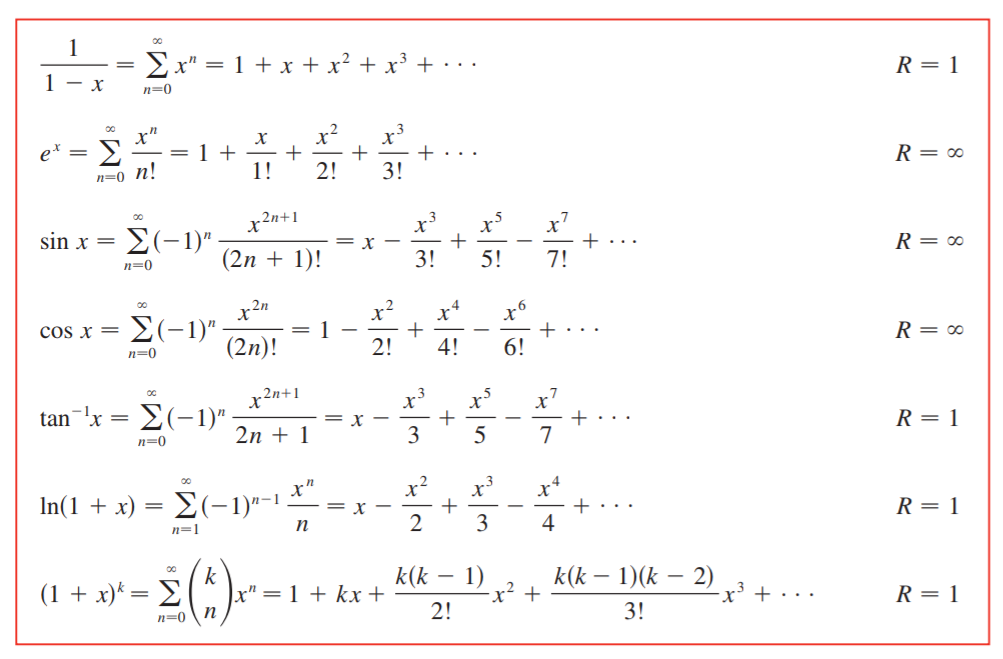
\includegraphics[width=0.9\linewidth]{seriesToFunctions.png}
        \end{figure}
        Using this, we can attempt to get a function into one of these forms, and then convert to the corresponding series. 

        \begin{mdframed}
            \textbf{Ex. } Find a series that represents $f(x) = \frac{1}{x+9}$.
            
            We will try to get this into the first form of the above table. 
            \begin{align*}
                =\frac {1}{x+9} = \frac{1}{9} \cdot \frac{1}{1-{-\frac{x}{9}}}
            \end{align*}
            Now we can convert this into a series. 
            \begin{align*}
                = \frac{1}{9} \cdot \sum_{n=0}^{\infty} \left(\frac{-x}{9}\right)^n = \frac{1}{9} \cdot \sum_{n=0}^{\infty} \frac{(-1)^n x^n}{9^n} = \sum_{n=0}^{\infty} \frac{(-1)^nx^n}{9^{n+1}}
            \end{align*}
        \end{mdframed}

    \section{Taylor and MacLaurin Series}
    If we \textbf{assume} that:
    \begin{align*}
        f(x)=c_0 + c_1 (x-a) + c_2 (x-a) + ... = \sum^{\infty}_{n=0} c_n (x-a)^n
    \end{align*}
    \textbf{Then:}
    \begin{align*}
        c_n = \frac{f^{(n)}(a)}{n!}
    \end{align*}

    We say that
    \begin{align*}
        \sum^{\infty}_{n=0} \frac{f^{(n)}(a)}{n!} (x-a)^n
    \end{align*}
    This is called the Taylor Series of $f$ centered at $a$. If $a=0$, we call it the MacLaurin series. 

    \begin{mdframed}
        \textbf{Ex. } Find the MacLaurin series of $f(x)=sin(x)$.
        
        We start by finding the pattern for $f^{(n)}(0)$. 
        \begin{figure}[H]
            \centering
            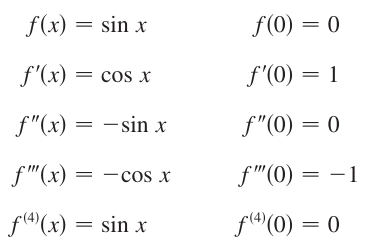
\includegraphics[width=0.4\linewidth]{sub.png}
        \end{figure}

        We see that each second term is 0, which means according to the definition of the MacLaurin series, ($c_n = \frac{f^{(n)}(a)}{n!}$), will kill that term. So we only have every second odd term.
        \begin{align*}
            x-\frac{x^3}{3!}+\frac{x^5}{5!}-\frac{x^7}{7!}+...=\sum^{\infty}_{n=0} (-1)^n \frac{x^{2n+1}}{(2n+1)!}
        \end{align*}
    \end{mdframed}

        \subsection{Binomial Series}
        The binomial series expansion is:
        \begin{align*}
            (1+x)^k = \sum^{\infty}_{n=0}\frac{k(k-1)(k-2)...(k-n+1)}{n!}\cdot x^n
        \end{align*}

    \section{Multi Variable Functions}
    A multi variable function is simply a function with more than 1 variable such as $f(x,y) = x+y + xy$.

    Just like single variable functions, multi variable functions have domains. 

    \begin{mdframed}
        \textbf{Ex. } Find the domain of $f$. 
        \begin{align*}
            z=f(x,y) = \frac{\sqrt{x-y+1}}{x-1}
        \end{align*}
        We see that $x\ne 1$ since that would cause the denomonator to be 0. Also, $x-y+1 > 0$ since we cannot take the root of a negative number. 

        That ends up being $y<x+1$. 

        We get the following graph:
        \begin{figure}[H]
            \centering
            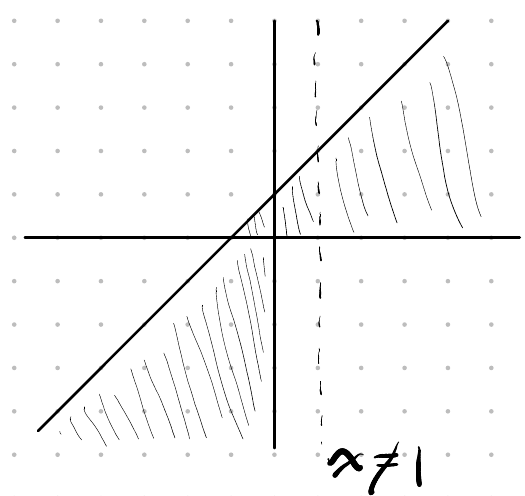
\includegraphics[width=0.4\linewidth]{ex1.png}
        \end{figure}
    \end{mdframed}

    We can also draw these graphs in 3D. To do this, we find the 2d graph at multiple $z$ coordinates, and then find the pattern. 

    \begin{mdframed}
        \textbf{Ex. } Draw the 3D Graph of $z=f(x,y)=\sqrt{x^2+y^2}$.

        We start by identifying the restrictions. $x^2 + y^2 \ge 0$. 
        
        Then we can draw the 2d graph at different $z$ values. We see that as $z$ increases, then the radius of the circle increases. (We see this by squaring both sides and getting $z^2 = x^2 + y^2$ which is the equation of a circle)

        Since it is a square root function, then if we set x or y to 0, and solve for z, we get $|x|$ or $|y|$. We therefore need to still show the absolute design on the graph. 

        Drawing this in 3D we get:
        \begin{figure}[H]
            \centering
            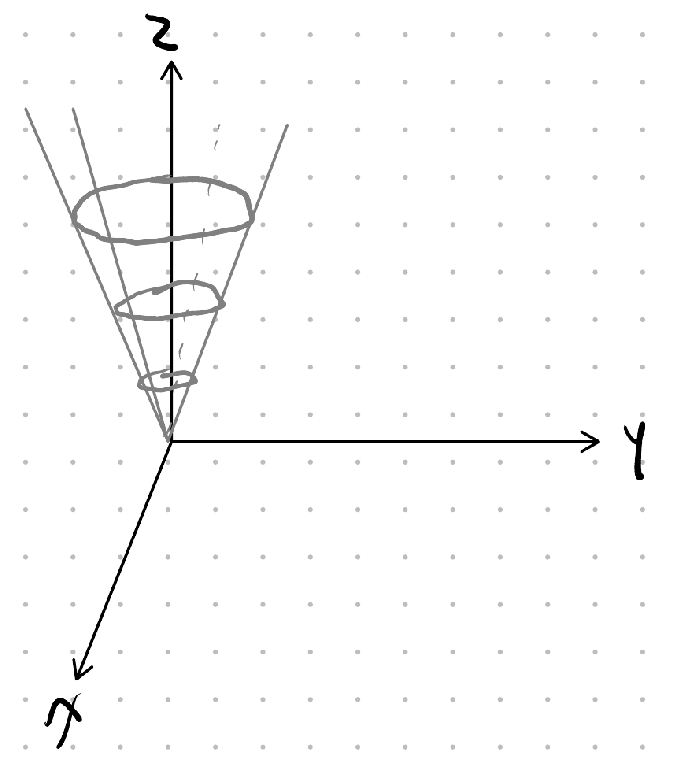
\includegraphics[width=0.4\linewidth]{ex2.png}
        \end{figure}
    \end{mdframed}

    A more systematic way to do this is to use the level curve. If we have $z=f(x,y)$, then we say the level curve of $f$ at height $c$ is:
    \begin{align*}
        L_c = \{(x,y)\in D | f(x,y)=c\}
    \end{align*}

    \begin{mdframed}
        Draw $L_2, L_4$ of $f(x,y) = x^2 + 2y^2$

        We start with the general formula: $L_c = \{(x,y) \in \mathbb{R} | x^2 + 2y^2 = c\}$

        Then we can adapt it for the 2 level curves. 
        \begin{align*}
            L_2 = x^2 + 2y^2 = 2\\
            L_4 = x^2 + 2y^2 = 4
        \end{align*}

        Both of those are just circles, so we can draw them. 

        \begin{figure}[H]
            \centering
            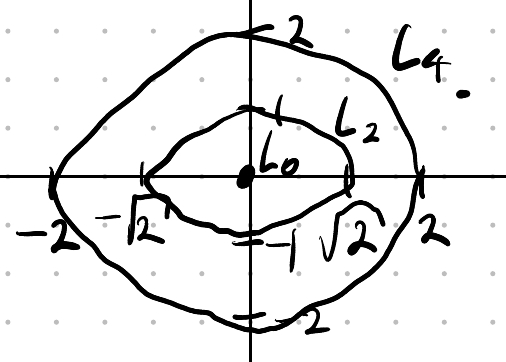
\includegraphics[width=0.4\linewidth]{ex3.png}
        \end{figure}
    \end{mdframed}

        \subsection{Partial Derivitives}
        For 1 variable functions, we just calculate 1 derivative. For 2 variable functions, we have 2 derivatives though denoted $f_x$ and $f_y$ or alternatively $\frac{\partial z}{\partial x}$ or $\frac{\partial z}{\partial y}$. 

        Basically when calculating $f_x$, we treat $x$ as a variable, and all other variables as constants. 

        We can also take second and third order derivatives, but we can do either $f_{xx}, f_{xy}, f_{yy}, f_{yx}$. Thankfully, $f_{xy} = f_{yx}$. So there are only 3 which is better than 4. 

        \begin{mdframed}
            \textbf{Ex. } Find $f_x(0,1)$ if $f(x,y) = \cos(x^2 - y^2) \cdot e^{x+y} - x^7y^3+x+y+1$

            We start by taking the derivative. We consider $y$ a constant.
            \begin{align*}
                f_x &= -\sin(x^2 - y^2)\cdot 2x\cdot e^{x+y} + e^{x+y}\cdot \cos(x^2-y^2) - 7x^6y^3+1\\
                f_x (0,1) &= \cos(-1)e+1
            \end{align*}
        \end{mdframed}

        \subsection{Tangent Planes}
        The 3D formula to calculate a tangent plane of a function $f(x,y)$ is:
        \begin{align*}
            z=f(a,b) + \frac{\partial f}{\partial x}(a,b) (x-a) + \frac{\partial f}{\partial y}(a,b)(y-b)
        \end{align*}

        \begin{mdframed}
            \textbf{Ex. } Find the equation of the tangent plane to the graph of:
            \begin{align*}
                z=f(x,y)=e^{x-y} + e^{x+y} + x^2 + y^2 + 1
            \end{align*}

            First we will find $f(0,1), f_x(0,1)$ and $f_y(0,1)$. I will skip lots of steps.
            \begin{align*}
                f(0,1) &= e^{-1}+e+2\\
                f_x(0,1)&=e^{-1} + e\\
                f_y(0,1) &= -e^{-1}+2+2
            \end{align*}

            Now we can simply plug it into the formula. 
            \begin{align*}
                z=(e^{-1}+e+2)+(e^{-1} + e)(x-0) + (-e^{-1}+2+2)(y-1) = \text{SIMPLIFY}
            \end{align*}
        \end{mdframed}

        \subsection{Linear Approximations}
        The equation for a linear approximation of $(x,y)$ is similar to the one for the tangent plane:
        \begin{align*}
            f(x,y)\approx L(x,y)=f(a,b) + \frac{\partial f}{\partial x}(a,b) (x-a) + \frac{\partial f}{\partial y}(a,b)(y-b)
        \end{align*}
        Note that $(x,y)$ is the actual point we are trying to find, and $(a,b)$ is a nicer point to work with that is close to $(x,y)$.

        \begin{mdframed}
            \textbf{Ex. } Estimate $f(-0.1,0.9)$ if :
            \begin{align*}
                z=f(x,y)=\sin(x-y)+e^{cos(x)y}-x-y+1
            \end{align*}

            First we need to pick a point that is close to $(-0.1, 0.9)$ and I will pick $(0,1)$. 

            So I need to find the tangent plane at $(0, 1)$.
            \begin{align*}
                f(0,1) &= \sin(-1)+e\\
                f_x(0,1) &=\cos(-1)-1\\
                f_y(0,1)&=-\cos(-1)+e-1
            \end{align*}

            Now I can sub that into the tangent plane / approximation equation.
            \begin{align*}
                L(a,b) = \sin(-1)+e + (\cos(-1)-1)(0-a)+(-\cos(-1)+e-1)(1-b)\\
                L(-0.1, 0.9) = \text{SUB IN AND SIMPLIFY}
            \end{align*}
        \end{mdframed}

        \subsection{Gradient Vector}
        We define the gradient vector $\vec{\nabla}f(x,y,z)$ as:
        \begin{align*}
            \vec{\nabla}f(x,y,z) = (f_x (x,y,z), f_y (x,y,z), f_z (x,y,z))
        \end{align*}
        In 2 dimensions, we just remove the $z$ coordinates from both sides. 

        \subsection{Directional Derivatives}
        We can find derivatives in directions other than just $x, y, z$. We use the following formula to find the directional derivative of $f$ in the direction of a \emph{unit vector }$u$.
        \begin{align*}
            D_{\vec{u}} f(a,b) = \vec{\nabla}f(a,b)\cdot (u_1, u_2)
        \end{align*}

        \begin{mdframed}
            \textbf{Ex. } Find $D_{\vec{u}} f(0,1)$ where $u = (1,1)$ and $f(x,y)=e^{xy}-e^{x+y}$.

            First we need to convert $u$ to a unit vector. 
            \begin{align*}
                |u| = \sqrt{1^2 + 1^2} = \sqrt{2} \implies \vec{u} = \left(\frac{1}{\sqrt{2}}, \frac{1}{\sqrt{2}}\right)
            \end{align*}

            After calculating the directional derivatives and then the gradient vector at (0,1), we get $\vec{\nabla}f(0,1) = (1-e, -e)$.

            Subbing these 2 pieces of information into the equation, and using the dot product, we get:
            \begin{align*}
                D_{\vec{u}}f(0,1) = (1-e, -e)\cdot \left(\frac{1}{\sqrt{2}}, \frac{1}{\sqrt{2}}\right) = \frac{1}{\sqrt{2}}(1-2e)
            \end{align*}
        \end{mdframed}

        We can get the following information of a directional derivative $D_{u} f(x,y)$:
        \begin{itemize}[noitemsep]
            \item The max is $|\vec{\nabla}f(x,y)|$ and occurs in the direction of $\vec{\nabla}f(x,y)$
            \item The min is $-|\vec{\nabla}f(x,y)|$ and occurs in the direction of $-\vec{\nabla}f(x,y)$
            \item It is $0$ if $\vec{u} \perp \vec{\nabla} f(x,y)$
        \end{itemize}

        \subsection{Chain Rule}
        \textbf{Assume} 
        \begin{align*}
            z=f(x_1, x_2, x_3, ..., x_n) \text{ and } x_j = g_j(t_1, t_2, t_3, ..., t_m) \text{ for } 1\le j\le n
        \end{align*}
        
        \textbf{Then}:
        \begin{align*}
            \frac{\partial z}{\partial t_i} = \frac{\partial z}{\partial x_1}\cdot \frac{\partial x_1}{\partial t_i} + \frac{\partial z}{\partial x_2}\cdot \frac{\partial x_2}{\partial t_i} + ... + \frac{\partial z}{\partial x_n}\cdot \frac{\partial x_n}{\partial t_i}
        \end{align*}

        \begin{mdframed}
            \textbf{Ex. } We have the following 4 functions. Find $\frac{\partial z}{\partial t}(1,1)$.
            \begin{align}
                z&=f(x_1, x_2, x_3) = x_1 x_3 + x_2\\
                x_1 &=x_1(s,t) = s+t\\
                x_2 &=x_2 (s,t) = e^s-t\\
                x_3 = x_3(s,t) = e_t-s
            \end{align}

            Recall that the formula states:
            \begin{align*}
                \frac{\partial z}{\partial t_i} = \frac{\partial z}{\partial x_1}\cdot \frac{\partial x_1}{\partial t_i} + \frac{\partial z}{\partial x_2}\cdot \frac{\partial x_2}{\partial t_i} + ... + \frac{\partial z}{\partial x_n}\cdot \frac{\partial x_n}{\partial t_i}
            \end{align*}
            Subbing in each partial derivitive we get:
            \begin{align*}
                \frac{\partial z}{\partial t} = (x_3)(1) + (1)(-1) + (x_1)(e^t) 
            \end{align*}
            Now we want it in terms of $s, t$ not $x_1, x_3$. So we sub those in to get:
            \begin{align*}
                = e^t - s - 1 + e^t (s+t) \implies \frac{\partial z}{\partial t} (1,1) = (e-1-1+2e) = 3e-2
            \end{align*}
        \end{mdframed}

        \subsection{Implicit Differentiation}
        We have the following 2 formulas:
        \begin{align*}
            \frac{\partial z}{\partial x} = \frac{\frac{-\partial F}{\partial x}}{\frac{\partial F}{\partial z}} \\
            \frac{\partial z}{\partial y} = \frac{\frac{-\partial F}{\partial y}}{\frac{\partial F}{\partial z}}
        \end{align*}

        Note that $F$ is the function $z=f(x,y,z) = 0$. Emphasis on the $=0$ part. 

        \begin{mdframed}
            \textbf{Ex. } Assume $e^x + e^{xy} + e^{xyz} = z$ defines $z$ implicitly as a function of $x,y$. Find $\frac{\partial z}{\partial y} (0,1,3)$.

            First we need to find $F$ by setting the function equal to 0.
            \begin{align*}
                F(x,y,z) = e^x + e^{xy} + e^{xyz} -z = 0
            \end{align*}

            Then we can go ahead and find $\frac{\partial F}{\partial y}$ and $\frac{\partial F}{\partial z}$. 
            \begin{align*}
                \frac{\partial F}{\partial y} = e^{xy}x + e^{xyz}xz \implies \frac{\partial F}{\partial y} (0,1,3) = 0\\
                \frac{\partial F}{\partial z} = e^{xyz}xy-1 \implies \frac{\partial F}{\partial z} (0,1,3) = -1
            \end{align*}

            Now we need to find $\frac{\partial z}{\partial y} (0,1,3)$ which is just the negative quotient of the 2 other partials that we found. 
            \begin{align*}
                \frac{\partial z}{\partial y} = \frac{\frac{-\partial F}{\partial y}}{\frac{\partial F}{\partial z}} = \frac{0}{-1} = 0
            \end{align*}
        \end{mdframed}

        

        


\end{document}